\section{語音數位內容檢索}
    
\subsection{簡介}
資訊檢索 (Information Retrieval) 系統一直以來都是研究人員與產業界關心的重點,但直到近年來由於網際網路、雲計算 (Cloud Computing) 的發達,使得網路上越來越多含語音資訊的多媒體檔案,我們稱之為語音數位內容 (Spoken Content),語音數位內容檢索的基本使用流程為:當使用者輸入了一段查詢詞 $Q$ (Query),系統會進行檢索並回傳按照相關性 (Relevance) 排序後的語音文件 $x$ (Spoken Documents)。此處每一篇文件與查詢詞的相關性被定義為 $S(Q, x)$,這個相關性函式通常是按照檢索系統的需求去決定的,可以是用機器學習 (Machine Learning) 的方法學習出來,也可以是由系統設計者決定。當系統接受到查詢詞 $Q$ 後,系統會計算每一篇文件 $x$ 與查詢詞 $Q$ 的相關性 $S(Q, x)$ 並排序後回傳給使用者,本篇論文中所使用的查詢詞 $Q$ 形式有二:文字構成的詞串、或口述形式。本篇論文使用的 $x$ 則都是語音文件。

\subsection{口述語彙偵測與語意檢索}
語音數位內容的檢索可以分為兩類:「口述語彙偵測 (Spoken Term Detection)」與「語意檢索 (Semantic Retrieval)」,口述語彙偵測回傳有出現查詢詞的語音文件,語意檢索則是回傳概念上相關的語音文件,而不一定要出現查詢詞,在此將兩者簡介如下: 

\subsubsection{口述語彙偵測}
口述語彙偵測的目的是檢索出所有包含查詢詞的語音文件,主要有兩種檢索情境。第一種是先將語音文件辨識為詞圖 (Lattice) 後,當使用者輸入文字的查詢詞後,系統會在詞圖上進行查詢詞的檢索。這種檢索情境需要有訓練好的自動語音辨識系統 (Automatic Speech Recognition, ASR),由於語音辨識系統並無法保證在所有情況下都有很好的辨識率,因此由辨識錯誤所導致的檢索性能下降是在此最需要解決的問題。過去的文獻有用聲學特徵如梅爾倒頻譜係數 (Mel-Frequency Cepstral Coefficients (MFCC)) 幫助分類器 (Classifier) 在分類一篇語音文件是否相關時的判斷,也有利用相關回饋 (Relevance Feedback)、圖論 (Graph) 與隨機漫步 (Random Walk) 解決這些問題。本論文中會應用到這類的檢索系統,計算此情境下的 $S(Q, x)$ 本章用到的方法為語言模型檢索法 (Langugage Modelling Approach),詳細方法列於~\ref{subsec:retrievalsystem}。

第二種是非監督式 (Unsupervised),的方法,查詢詞與語音文件都是語音形式的,也有人稱之為依例查詢 (Query-by-Example),系統直接利用如動態時間校準 (Dynamic Time Warping) 等方法在信號上比對語音文件中是否有某一段聲音與查詢詞很相像,過去的方法通常是為了解決不同文件間語速上的差異提出如有斜率限制的動態時間校準 (Slope-Constraint DTW),或是為了解決動態時間校準逐一比對所有文件庫所花時間過多的問題。本論文中會應用到這類的檢索系統,計算此情境下的 $S(Q, x)$ 為利用片段式動態時間規劃 (Segmental Dynamic Time Warping),簡介於~\ref{sec:chap4_sdtw}。

\subsubsection{語意檢索}
時至今日,大部分的語音數位內容檢索的研究是專注於口述語彙偵測的,但是這是不夠的,因為使用者通常希望查詢結果與自己輸入的查詢詞是概念上匹配 (Concept Matching) 的,而不是只回傳有出現查詢詞的文件,比如當使用者查詢「東京旅遊」,他可能期待查到包含「東京旅館」、「東京鐵塔」的文件,而不是與查詢詞完全一樣的文件。文字領域的資訊檢索已經有「概念匹配」的做法來達到語意檢索,但是由於文字領域的資訊檢索是在文字為完全正確的狀況下,不像語音數位文件的檢索往往會有辨識錯誤的問題,因此本論文提出了利用自動尋找的聲學組型來解決這個問題,語意檢索也是本論文的主軸。一個較常見的實作方法通常是使用相關回饋 (Relevance Feedback) 與查詢詞擴展 (Query Expansion),分別介紹於~\ref{sec:pseudo_feedback}和~\ref{sec:query_doc_exp}。

\subsection{詞圖與唯一最佳序列}
當給定了一段語音文件,自動語音辨識系統 (Automatic Speech Recognition, ASR) 能夠將這段語音文件辨識成兩種格式:詞圖 (Lattice)~\cite{saraclar51lattice} 與唯一最佳序列 (One-Best Transcription),本論文中兩種形式的辨識格式都會使用,故介紹如下:

詞圖像張網一樣,如圖 ~\ref{fig:chap2_lattice},將每個時間所有可能的詞都呈現出來,而唯一最佳序列只呈現了詞圖上一條最可能的詞串當作辨識結果而已。通常在語音檢索時會使用詞圖來搜尋,因為語音辨識通常沒有辦法做到完全準確,可能會辨識成音很像的其他詞彙,比如「美國」可能會被辨識成「沒過」等等,如果使用唯一最佳序列的話,選中了正確的詞彙固然很好,但如果沒選中就會完全搜尋不出來了,而使用詞圖的話,即使唯一最佳序列被辨識錯了,通常正確的詞彙都還是會被表示在詞圖上,所以一般來說會使用詞圖來表示辨識的結果。

\begin{figure}
\centering
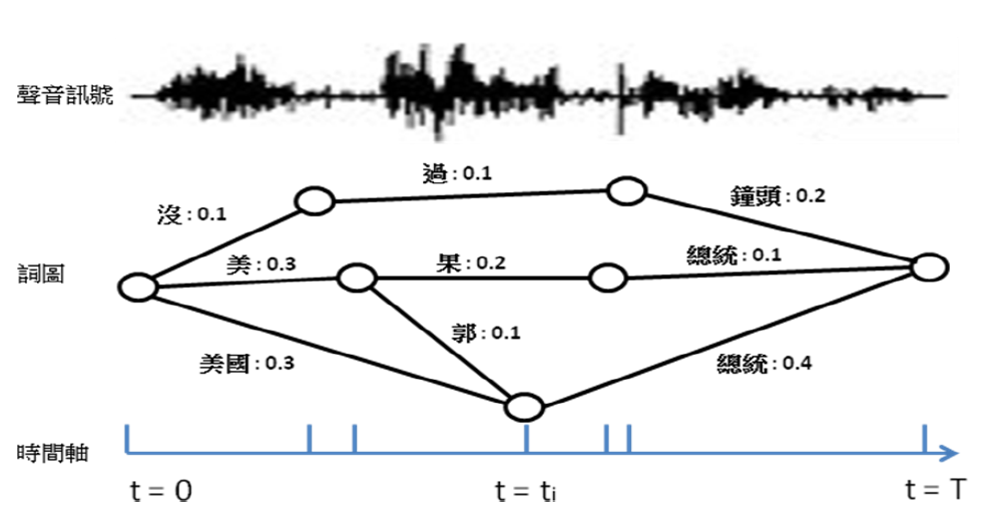
\includegraphics[scale=0.5]{images/chap2_lattice.png}
\caption{詞圖示意圖} \label{fig:chap2_lattice}
\end{figure}

如圖~\ref{fig:chap2_lattice}所示,詞圖主要由${N, A}$所構成,其中$N$是所有節點 (Node) 的集合,而$A$則是所有的詞弧 (Word Arc) 的集合。節點上存有各節點的時間資訊,而詞弧上除了有起始節點和終止節點外,還包含了在這個詞弧上的假設詞 (Word Hypothesis) 與此假設詞的信心分數 (Confidence Score) ,而此假設詞和信心分數都是由聲學模型和語言模型所計算出來的。

語音辨識系統的輸入是聲學特徵,並找出最有可能的詞彙串。因此相當於最大化以下的式子:
    \begin{equation}
    w^*_{seq} = argmax_{w_{seq} \in W_{seq}}P(w_{seq}|O)
    \end{equation}
O為輸入訊號之聲學特徵,$w_{seq}$為某個詞串,$W_{seq}$為所有$w_{seq}$之組合,$argmax$則是尋找一個$w_{seq}$使得$P(w_{seq}|O)$最大,此$w_{seq}$即為$w^*_{seq}$。但$P(w_{seq}|O)$無法直接計算,所以根據貝氏定理 (Bayes' Theorem),可以表示如下:
    \begin{equation}
    P(w_{seq}|O) = \frac{P(O|w_{seq})P(w_{seq})}{P(O)}
    \end{equation}
由於$P(O)$對固定的$O$是常數,可以不考慮,上式可簡化成:
    \begin{equation}
    P(w_{seq}|O) = P(O|w_{seq})P(w_{seq})
    \end{equation}

可以看得出來,$P(O|w_{seq})$可以由聲學模型求得,$P(w_{seq})$可以從語言模型中求得。求出來的$w^*_{seq}$即為唯一最佳序列。有時也會使用N最佳序列 (N-Best List) ,概念與唯一最佳序列很像,只是找出前N個讓$P(w_{seq}|O)$ 最大的$w_{seq}$。

\subsection{辭典外詞彙 (Out of Vocabulary)}
由於自動語音辨識系統可以辨識出的字彙在自動語音辨識系統被訓練時就被決定好了,因此當系統要辨識新的詞彙的時候,如果這套系統在辨識時遇到辭典中沒有的詞彙時,系統就無法辨識出來,此問題稱為辭典外詞彙問題 (Out of Vocabulary Problem)。如此一來,如果檢索系統發現查詢詞是辭典外詞彙,則這段查詢詞就無法被辨識,進而使得檢索系統的成效下降,更糟糕的是,由於查詢詞往往會是較少見的字彙,因此查詢詞是辭典外詞彙的機率有時會超過$15\%$。

一個常見的解決辦法是使用次詞單位 (Subword Units)。先建立一套自動語音辨識系統,而這套系統是將聲音辨識成次詞單位的唯一最佳序列或是詞圖,當查詢詞進來後,也是將查詢詞轉換為次詞單位,之後系統再比對次詞單位的辨識結果與查詢詞的次詞單位版本,而在這套系統下,通常會需要字形轉音素的系統 (Grapheme-to-phoneme),使得這個作法變得較為困難。

以詞為基礎的檢索 (Word-based) 和以次詞單位為基礎的檢索 (Subword-based) 各有優缺,詞的檢索會遇到很多辭典外詞彙的問題,使得檢索系統的成效大幅下降,而次詞單位為基礎的檢索則能提高召回率 (Recall),但由於次詞單位不是代表字義的最小單位,因此檢索回來的文件準確率則會下降。所以比較好的方法是同時使用詞為基礎的檢索和以次詞單位為基礎的檢索,系統同時利用詞和次詞單位進行檢索,並將兩者的檢索結果進行疊加 (Interpolation),此方法需要決定疊加時的權重,而此權重通常可以利用一套查詢詞的訓練集完成,本論文中的檢索也是同時使用詞與次詞單位為基礎的檢索。

\subsection{檢索系統}
\subsubsection{計算文字查詢詞與詞圖的相關性 $S(Q, x)$ (使用語言模型檢索)}
\label{subsec:retrievalsystem}
檢索系統的目的主要是當使用者輸入查詢詞$Q$時,系統能夠計算出每個文件$x$與查詢詞間的相關分數$S(Q, x)$,進而將此相關分數排序後回傳給使用者。當系統接收到語音訊號時,系統會先對其抽取出聲學訊號,再經過聲學模型和語言模型辨識成唯一最佳序列或詞圖,一般來說,語音檢索系統使用詞圖的表現會比較好,所以以下主要就如何計算出查詢詞和詞圖的相關分數$S(Q, x)$加以介紹。

由於本章使用的檢索方式是語言模型檢索 (Language Modelling Retrieval)~\cite{zhai2008statistical, chia2010statistical},因此首先要把辨識所得的詞圖轉換為語言模型。對每個詞圖中的詞$t$,它在詞圖中的期望出現次數 (Expected Count) 可以如此計算:

\begin{equation}
E[t|x] = \sum_{\mu \in L(x)} N(t, \mu)P(\mu|x)
\end{equation}

$L(x)$是$x$的詞圖中所有的路徑,$\mu$是$L(x)$中的一條路徑,$N(t, \mu)$是$t$在$\mu$中出現的次數,$P(\mu|x)$是路徑$\mu$的事後機率(Posterior Probability)。

有了$E[t|x]$之後,就能把詞圖表示成單連詞 (Uni-gram) 語言模型$\theta_x$:

\begin{equation}
P(t|\theta_x) = \frac{E[t|x]}{\sum_tE[t|x]}
\end{equation}

因為$\theta_x$裡沒有包含每個詞,為了讓$\theta_x$中每個詞都有一點機率,會再把$\theta_x$與一個背景語言模型 (Background Language Model) $\theta_b$做線性疊加,此過程稱為平滑化 (Smoothing)~\cite{zhai2001study},$\theta_b$可以如此估計:

\begin{equation}
P(t|\theta_b) = \frac{\sum_{x\in C}E[t|x]}{\sum_t\sum_{x\in C}E[t|x]}
\end{equation}

$C$ 是所有文件$x$的集合。

同樣地,查詢詞$Q$也可以被表示成語言模型$\theta_Q$:

\begin{equation}
P(t|\theta_Q) = \frac{N(t, Q)}{|Q|}   
\end{equation}

$N(t, Q)$是詞$t$出現在$Q$中的次數,而$|Q|$是$Q$中詞的總數。

有了$\theta_x, \theta_b, \theta_Q$之後,就可以計算$\theta_x$與$\theta_Q$之間的相關分數$S(x, Q)$了,由於$\theta_x, \theta_b, \theta_Q$都是機率分布 (Probability Distribution) ,所以在這裡選擇了KL散度 (Kullback–Leibler divergence) 用來計算兩個語言模型之間的距離,KL散度的計算方式如下:

\begin{equation}
KL(\theta_x | \theta_Q) = \Pi_{w\in V}P(w|\theta_x)^{P(w|Q)}
\end{equation}

於是定義文件$x$和查詢詞$Q$之間的相關分數$S(x, Q)$如下:

\begin{equation}
S(x, Q) = -[(1-w_1)KL(\theta_q^w|\bar{\theta}^w_x) + w_1KL(\theta_q^s|\bar{\theta}_x^s)]
\end{equation}

$\bar{\theta}_x$是將$\theta_x$與$\theta_b$疊加後的語言模型,上標$w$代表的是用以詞為基礎的詞圖產生的語言模型,上標$s$代表的是用以次詞 (Subword) 為基礎的詞圖產生的語言模型,上式是分別對詞為基礎的語言模型和次詞為基礎的語言模型做檢索,再將兩者得到的相關分數用$w_1$做線性疊加,最後再將此分數排序後回傳給使用者。

\subsection{片段式動態時間校準 (Segmental DTW)}
\label{sec:chap4_sdtw}
口述語彙偵測的目的是要搜尋整個語料庫後,找出其中有出現查詢詞的語音文件,並且找出這些語音文件中可能有出現查詢詞的假設區域 (Hypothesized Region) ,並給這個假設區域一個相關分數,最後系統再根據相關分數進行排序後回傳給使用者 (分數較高為較相關)。

這裡考慮的口述語彙偵測是查詢詞也是語音形式的情境。此時所用的方法為片段式動態時間校準 (Segmental Dynamic Time Warping)~\cite{chan2010unsupervised, hazen2009query}。假設輸入的查詢詞的特徵為$\mathbf{X} = (\mathbf{x}_1, ..., \mathbf{x}_{|\mathbf{X}|})$,語音文件的特徵為$\mathbf{Y} = (\mathbf{y}_1, ..., \mathbf{y}_{|\mathbf{Y}|})$,有了這兩者之後,就可以建立一個距離表格 (Distance Table) $D(i, j) = \rho(\mathbf{x}_i, \mathbf{y}_j)$,通常這裡使用的特徵是
高斯事後機率 (Gaussian Posteriorgrams)~\cite{zhang2009unsupervised}或是梅爾倒頻譜係數 (MFCC)。如果使用高斯事後機率的話,兩個音框之間的距離為 $\rho(\mathbf{x}_i, \mathbf{y}_j) \equiv -\log (\mathbf{x}_i \cdot \mathbf{y}_j)$。如果使用梅爾倒頻譜係數的話,兩個音框之間的距離為兩點之間的歐幾里得距離 (Euclidean Distance),即$\rho(\mathbf{x}_i, \mathbf{y}_j) \equiv \sqrt{|\mathbf{x}_i - \mathbf{y}_j|^2}$

動態時間校準的目的是要在 $D(i, j)$ 上找一條距離總合最短的路徑從 $(1, s)$ 到 $(|\mathbf{X}|, e)$ 表示從 $\mathbf{X}$對應到$(\mathbf{y}_s, ..., \mathbf{y}_e)$ (因為查詢詞一定要被完全對應,而語音文件不一定要被完全對應到)。由於假設區域可以出現在語音文件中的任何地方, 因此片段式動態時間校準將距離表格 $D(i, j)$ 切成數個重疊的對角片段 (寬度為 $R$),所以說每個片段的起始點分別為 $(1, 1), (1, 1+R), (1, 1+2R),...$ 如圖 ~\ref{fig:chap4_sdtw} 所示,每個對角片段都代表了一個可能出現查詢詞的區域,所以要在每個對角片段上找出距離總合最短的路徑,即這個對角片段上的假設區域。片段式動態時間校準會從每個片段中找出一段距離總合最短的路徑,在每個片段中所有對應的路徑 (Warping Path) 都必須要完整地待在片段內,不可超出片段。

\begin{figure}
\centering
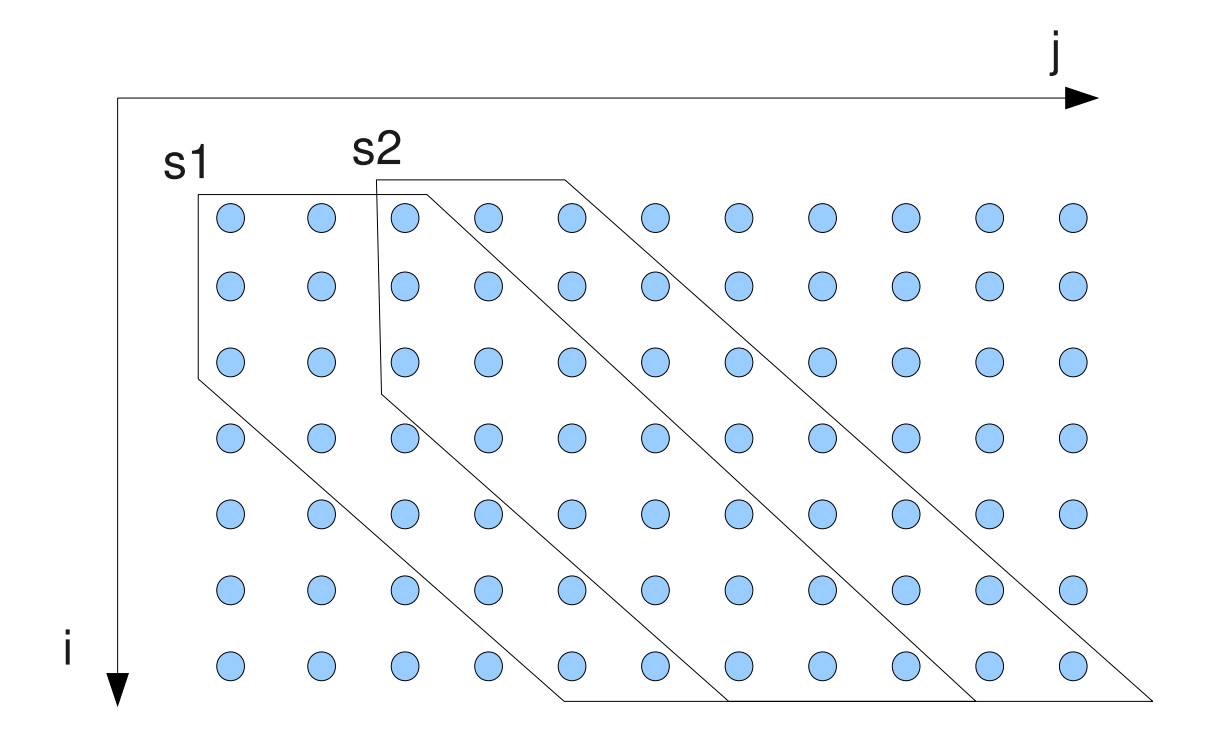
\includegraphics[scale=0.3]{images/chap4_sdtw.png}
\caption{片段式動態時間校準示意圖~\cite{zhang2009unsupervised}} \label{fig:chap4_sdtw}
\end{figure}

假設在每個片段中的對應路徑為:

\[
\phi = (i_t, j_t), t = 1,...,|\phi|
\]

代表著如下的對應關係:

\[
\mathbf{x}_{i_1} \leftrightarrow \mathbf{y}_{j_1}, \mathbf{x}_{i_2} \leftrightarrow \mathbf{y}_{j_2},...,\mathbf{x}_{|\phi|} \leftrightarrow \mathbf{y}_{|\phi|},
\]
而邊界條件是 $i_1 = 1, i_{|\phi|} = |\mathbf{X}|$ ,$j_1$ 為 $1+kR$ ,對應路徑中所有的點都要在片段內,即:

\[
|(i_t-i_1)-(j_t-j_1)| <= R
\]

而片段式動態時間校準的目標是要在每個片段內找到一條路徑 $\phi$ 使得下式的距離總和最小:

\begin{equation}
C_{\phi}(\mathbf{X}, \mathbf{Y}) = \sum_{t=1}^{|\phi|} \rho(\mathbf{x}_{i_t},\mathbf{y}_{j_t})
\end{equation}

\begin{figure}
\centering
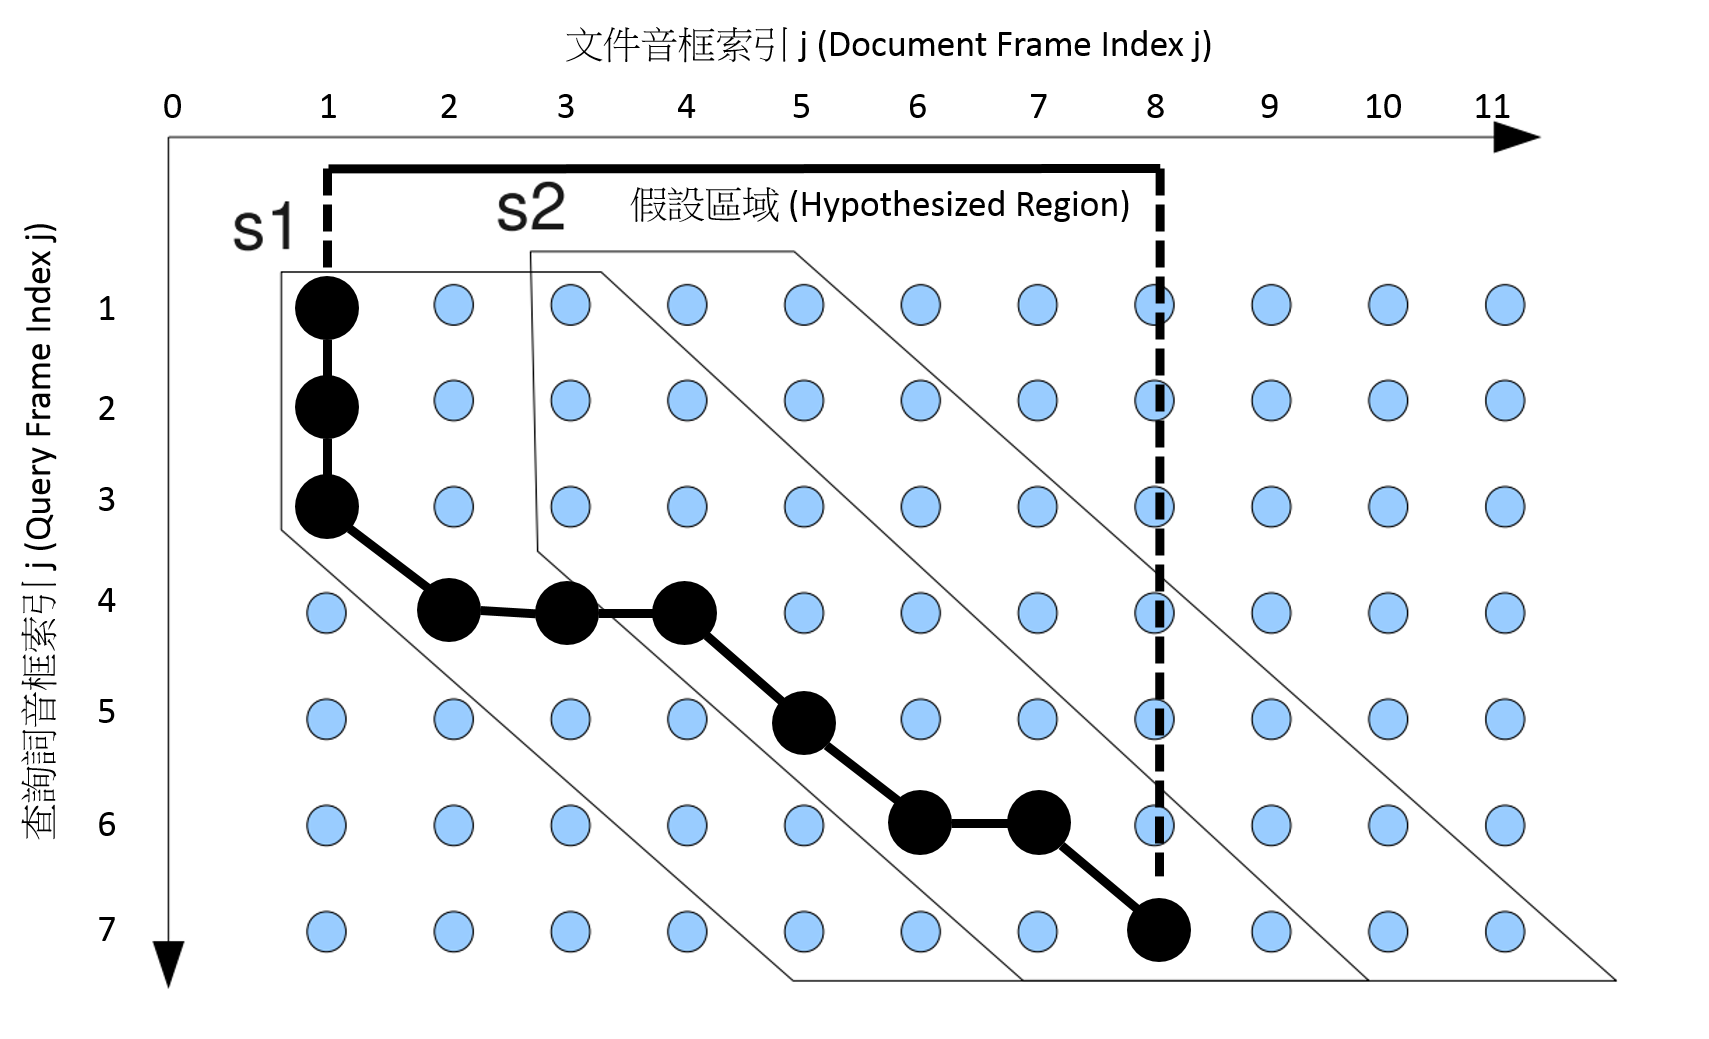
\includegraphics[scale=0.45]{images/chap2_segdtw_exp1.png}
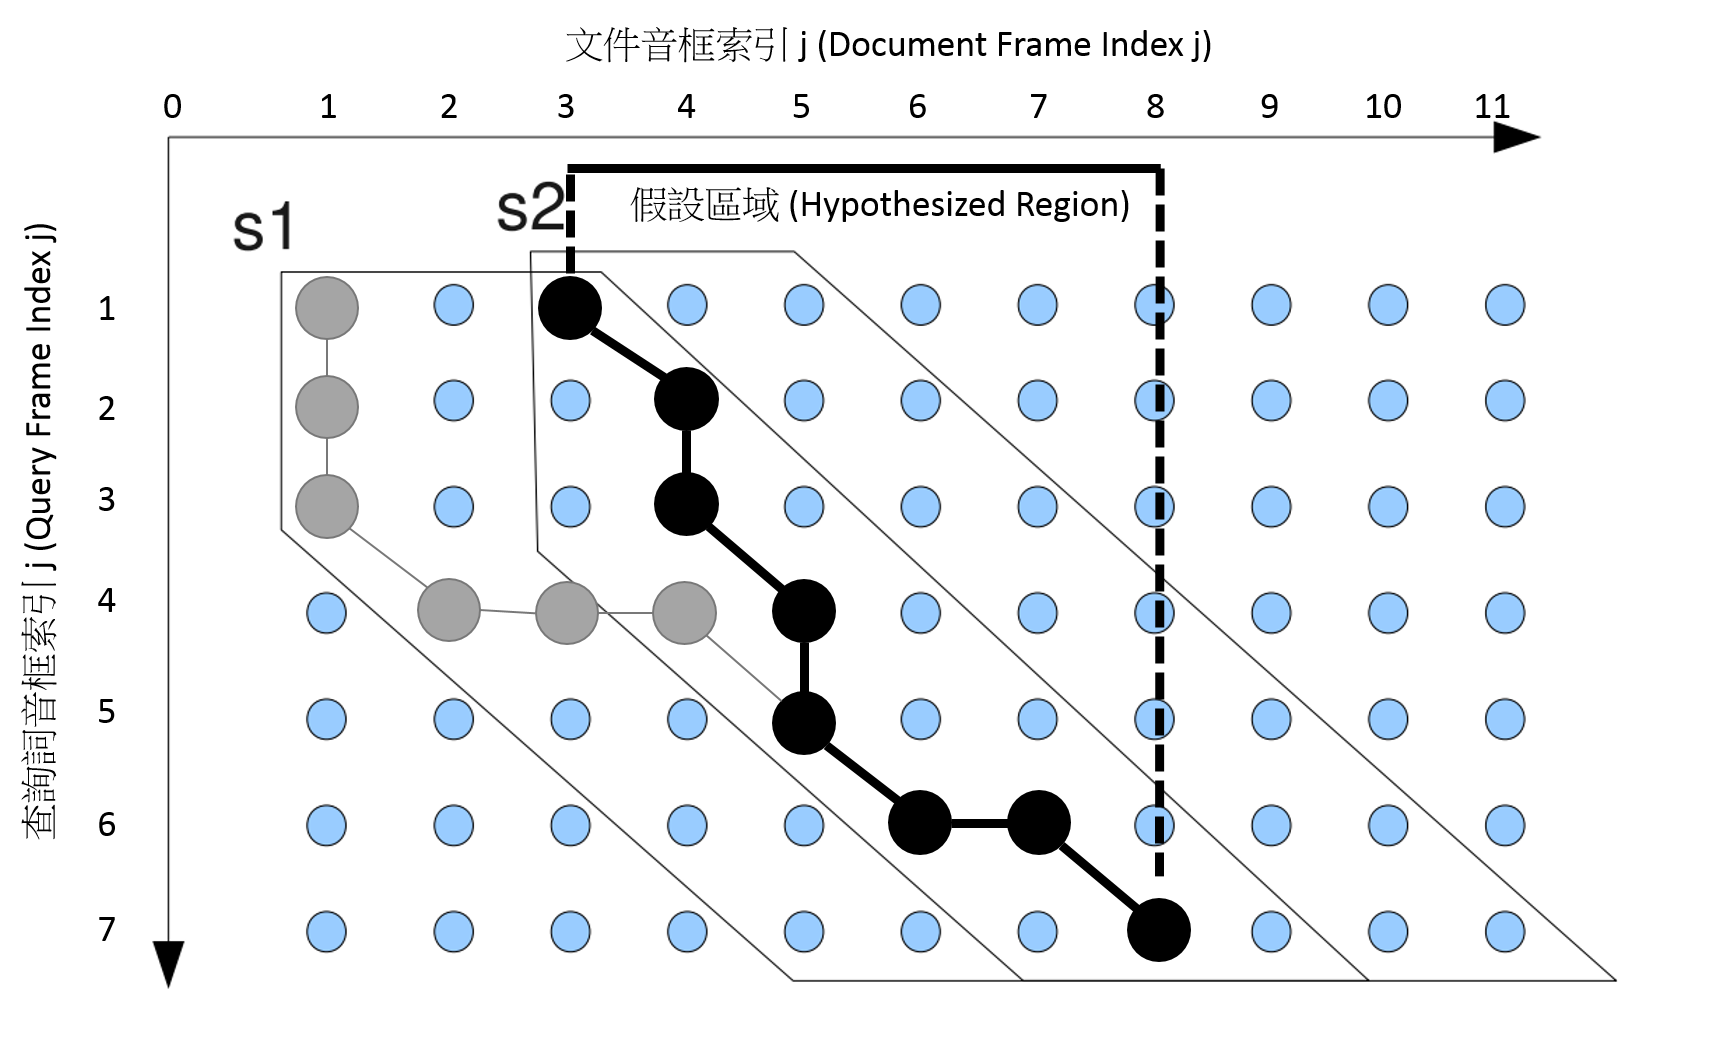
\includegraphics[scale=0.45]{images/chap2_segdtw_exp2.png}
\caption{示意如何從兩個對角片段中找到相關分數最大的假設區域,其中 $R=2$}
\label{fig:chap2_sdtw_exp}
\end{figure}


每個片段中使得 $C_{\phi}(\mathbf{X}, \mathbf{Y})$ 最小,即使得相關分數 $-C_{\phi}(\mathbf{X}, \mathbf{Y})$ 最大的那條 $\phi$ 即為每個片段中的假設區域 $(\mathbf{y}_{j_1},...,\mathbf{y}_{j_{|\phi|}})$ ,而在每個片段中找到最大相關分數的路徑可以使用動態規劃 (Dynamic Programming) 求解。圖~\ref{fig:chap2_sdtw_exp}中顯示了兩個對角片段與其對應的最大相關分數的路徑與假設區域。圖中上半部中的 $(\mathbf{y}_1, ..., \mathbf{y}_8)$ 代表在第一個對角片段中找到的假設區間,圖中下半部中的 $(\mathbf{y}_3, ..., \mathbf{y}_8)$ 則是在第二個對角片段中找到的假設區域。 找到所有假設區域後,將假設區域按照其與查詢詞的相關分數進行排序後,即為口述語彙偵測的結果。在一篇語音文件中找到所有可能的假設區域需要 $O(|\mathbf{X}||\mathbf{Y}|)$ 的計算量來計算點與點之間的距離 $\rho$,並需要$O(|\mathbf{X}||\mathbf{Y}|)$的計算量來找到相關分數最大的路徑。

\subsection{資訊檢索評估機制}
為了讓研究人員能夠比較彼此系統之成效,制定資訊檢索評估機制的標準是很重要的一環,本節將介紹此篇論文使用的評估機制。

\subsubsection{準確率(Precision)與召回率(Recall)}

準確率越高代表所找出的檢索結果越可靠,而召回率越高的話代表系統找回越多相關的檢索目標,通常會為系統設定一個閥值(Threshold),文件的分數若高於閥值,則視為相關,反之若文件的分數低於閥值,則視為不相關。準確率和召回率的定義如下:

\[
\text{準確率}=\frac{\text{檢索到的相關檢索對象數}}{\text{檢索到的檢索對象數}}
\]

\[
\text{召回率}=\frac{\text{檢索到的相關檢索對象數}}{\text{所有的相關檢索對象數}}
\]

通常這兩個值彼此之間的關係為負相關。調高閥值的話準確率會上升,但召回率則會下降;反之若調低閥值,準確率會因此下降,召回率則會很高。可以考慮一個極端例子:當閥值非常低時,幾乎所有的文件都是相關文件,此時的召回率相當於1,但準確率就會很低了。因此單看準確率或召回率是無法準確地評估系統的優劣的,必須要兩者一起評估。

\begin{figure}
\centering
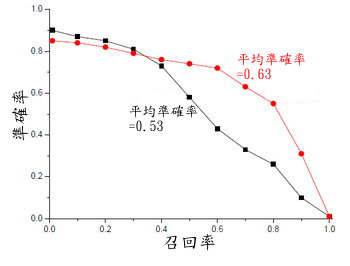
\includegraphics[scale=1.0]{images/chap2_precision_recall.png}
\caption{準確率、召回率和平均準確率之關係} \label{fig:precision_recall}
\end{figure}

\subsubsection{P@N}

通常使用者最重視的是檢索系統傳回的前幾名結果,所以就發展出了$P@N$這個評估機制。$P@N$就是只看前N個檢索結果的正確率。例如:前五個檢索結果中有一個是相關的,那$P@5$就是20\%。

$P@N$的定義如下:
\[
P@N=\frac{\text{前N個文件裡的相關文件數}}{N}
\]

\subsubsection{平均準確率~\cite{garofolo2000trec}}

因為準確率和$P@N$都需要事先決定,當查詢詞和條件不同時,很難準確地評估兩個系統的效能。因此有人提出了平均準確率(Mean Average Precision, MAP)的概念,如圖~\ref{fig:precision_recall},平均準確率就是準確率和召回率曲線下面積的平均值。平均準確率的定義如下:
\begin{equation}
MAP = \frac{1}{|Q|} \sum_Q \frac{\sum_{d \in D^R}precision(d)}{|D^R|}
\end{equation}
其中Q代表查詢詞的集合,$|Q|$為查詢詞的總數,$D^R$為和查詢詞Q相關的文件d的集合,$|D^R|$代表和查詢詞Q相關的文件數量。precision(d)代表系統檢索出文件d時的準確率。

\section{相關回饋}
相關回饋 (Relevance Feedback) 是資訊檢索的一項重要的技術~\cite{ruthven2003survey},通常可以顯著地提升系統的成果。相關回饋基本的架構如圖 ~\ref{fig:chap2_prf},使用者輸入查詢詞之後,系統會先根據查詢詞與所有文件的相關分數 $S(Q, d)$ 排序出第一次檢索結果 (First-pass Result)。然後把第一次檢索結果中部分文件標注為與查詢詞相關的正例 (Positive Example) ,部分文件標注為與查詢詞非相關的反例 (Negative Example)
,系統會再根據標注的結果重新計算查詢詞與文件的關係,把調整後的結果呈現給使用者看。
\begin{figure}
\centering
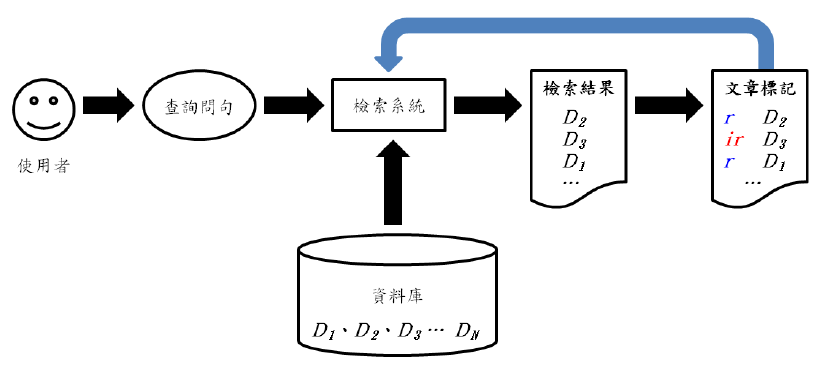
\includegraphics[scale=0.7]{images/chap2_prf.png}
\caption{相關回饋的基本架構} \label{fig:chap2_prf}
\end{figure}


把部分文件標注成正例與反例的方法可以大致分為以下幾種:

\subsection{外顯回饋}
外顯回饋 (Explicit Feedback) 的做法通常是由使用者告訴系統文件是否為正例或反例,進而增進檢索的成果。外顯回饋可分為使用者回饋 (User Feedback) 和積極回饋 (Active Feedback)
,使用者回饋是由使用者依據第一次檢索結果按照文件相關性進行標注~\cite{salton1975vector, zhai2001model, robertson1976relevance};積極回饋則是由系統主動詢問使用者某文件為正例或反例(通常是系統無法決定的文件),此方法可以盡量減少使用者的標注量以改進系統的成果~\cite{tong2001support, goh2004multimodal, he2004mean}。

\subsection{隱含回饋}
隱含回饋 (Implicit Feedback) 是不由使用者直接提供正反例的資訊,而且透過觀察使用者的行為 (Behavior) 而分析文件的相關性,因此使用者並不知道自己正在回饋給系統。最常用的方法是點擊數據 (Click-through Data),比如檢索系統的前幾名如果是$d_1, d_2, d_3, ...$,而使用者沒有檢視$d_1$,而是直接檢視$d_2$,如此一來系統就可以假設$d_1$是不相關的文件,而$d_2$是相關的文件。除此之外,還可以利用查詢記錄 (Query Log)、網頁捲動
(Scrolling)和滑鼠軌跡 (Mouse Movements) 等~\cite{kelly2003implicit}。

\subsection{虛擬回饋}
\label{sec:pseudo_feedback}
虛擬回饋 (Pseudo Feedback) 不需要使用者的參與,在系統產生第一次檢索結果後,系統會直接假設其中某些部分為正例,某些部分為反例(通常是直接假設相關分數最高的$N$篇為正例,相關分數最低的$N$篇為反例)。系統會再根據這些假設進行進一步的檢索,在這個過程中,系統雖然沒有得到額外的資訊,但系統的成效通常能有一定的提升~\cite{kurland2005better, xu1996query, yu2003improving, sakai2005flexible, cao2008selecting, lee2008cluster, lv2009comparative, lv2010positional},而虛擬回饋也是此篇論文的主要研究主題之一。

\subsection{查詢詞擴展與文件擴展}
\label{sec:query_doc_exp}
語意檢索最大的困難點是由於最理想的檢索結果不一定要包含查詢詞,假設查詢詞是「東京旅遊」,則包含「東京鐵塔」的文件的 $S(Q, d)$ 則會非常低,常見的解決方法是使用查詢詞擴展 (Query Expansion) 和文件擴展 (Document Expansion),一個是將許多與查詢詞語義上相關的詞加入原查詢詞中成為新的查詢詞模型,另一是將文件加入更多語義上相關的詞,這裡使用的是潛藏語意分析 (Probabilistic Latent Semantic Analysis, PLSA) 來找到與語義上相關的詞。這兩個方法都能解決查詢詞與文件中詞彙不匹配的問題,以下將分別介紹:

\subsubsection{查詢詞擴展 (Query Expansion)}
\label{sec:prf}
這裡使用正規化查詢詞混合模型 (Query-Regularized Mixture Model) 作為查詢詞擴展的實作方法,這套方法假設每篇文件都是由查詢詞相關詞彙 (Query-Related Terms) 和一般詞彙 (General Words)
所組成,而這兩者的比例在每篇文件中都是不一樣的。舉例來說,當一篇實際上不相關的文件被錯誤地假設成虛擬相關文件時,這個比例應該要很低,而反之亦然。然而實際上這個比例是不知道的,不過可以從虛擬相關文件中估計出來這個比例,估計完之後新的查詢詞模型稱為 $\theta_Q^{'}$,用來取代原本的 $\theta_Q$。

假設所有的文件為集合 $D$,其中包含了文件 (已經過第一次檢索排序後) ${d_1, d_2, ..., d_n, ...}$,因此虛擬相關的文件為 ${d_1, d_2, ..., d_m, ..., d_M}$,而 $M$ 是虛擬相關文件的總數。每一篇文件中的詞都可以看作是由背景語言模型 (Background Language Model) $\theta_b$ 產生,或是由新的查詢詞模型 $\theta_Q^{'}$ 產生,$\alpha_{d_m}$是$d_m$這篇文件中詞彙由 $\theta_Q^{'}$ 產生的機率,反之 $(1-\alpha_{d_m})$ 則是由背景模型 $\theta_b$ 產生的機率。透過最大概似估計最大化下式即可以估計出
$\theta_Q^{'}$ 和每一篇 $d_m$ 的 $\alpha_{d_m}$:

\begin{equation}
\label{equ:chap2_prf_f1}
F_1(\theta_Q^{'}, \alpha_{d_1}, ..., \alpha_{d_M}) = \Pi^M_{m=1} \Pi_w (\alpha_{d_m} P(w|\theta_Q^{'}) + (1 - \alpha_{d_m}) P(w|\theta_b))^{P(w|\theta_{d_m})}
\end{equation}

上式中,產生詞彙 $w$ 的機率為 $\alpha_{d_m} P(w|\theta_Q^{'}) + (1-\alpha_{d_m}) P(w|\theta_b)$ 。因此上式可視為由新的查詢詞模型產生這些虛擬相關文件的可能性 (Likelihood)。然而,如果只最大化式~\ref{equ:chap2_prf_f1},$\theta_Q^{'}$ 中主要會包含這些虛擬相關文件的主題,而不一定是查詢詞相關的詞彙,為了要解決這個問題,比較好的方法是用原本的查詢詞模型 $\theta_Q$ 正規化 (Regularize) $\theta_Q^{'}$,因此定義 $F_2(\theta_Q^{'})$ 如下:

\begin{equation}
\label{equ:chap2_prf_f2}
F_2(\theta_Q^{'}) = \Pi_w P(w|\theta_Q^{'})^{P(w|\theta_Q)}
\end{equation}

當 $\theta_Q^{'}$ 與 $\theta_Q$ 越近時,$F_2(\theta_Q^{'})$的值會越大。

有了式~\ref{equ:chap2_prf_f1}和式~\ref{equ:chap2_prf_f2}後,只要最大化下式即可估計 $\theta_Q^{'}$ 和 $\alpha_{d_m}$ :

\begin{equation}
\label{equ:chap2_prf_f1f2}
F(\theta_Q^{'}, \alpha_{d_1}, ..., \alpha_{d_M}) = F_1(\theta_Q^{'}, \alpha_{d_1}, ..., \alpha_{d_M}) F_2(\theta_Q^{'})^\lambda
\end{equation}

$\lambda$ 是個用來控制 $F_2(\theta_Q^{'})$ 影響力的參數,$\lambda$ 越大,新的查詢詞模型 $\theta_Q^{'}$ 就會跟原本的查詢詞模型 $\theta_Q$ 越像。最大化式~\ref{equ:chap2_prf_f1f2} 的好處是新的查詢詞不會過適 (Overfit) 到虛擬文件,而會保留與原本的查詢詞模型 $\theta_Q$ 一定程度的相似性。	

最大化式 ~\ref{equ:chap2_prf_f1f2} 可以採用 EM 演算法 (Estimation-Maximization Algorithm):

E step: 對於${d_1, d_2, ..., d_M}$ 中的每篇文件$d_m$中的每一個詞彙 $w$:

\begin{equation}
\label{equ:chap2_prf_estep}
P(R|w, d_m) = \frac{\alpha_{d_m} P(w|\theta_Q^{'})}{\alpha_{d_m} P(w|\theta_Q^{'}) + (1-\alpha_{d_m}) P(w|\theta_b)}
\end{equation}

其中 $P(R|w, d_m)$ 為當給定文件 $d_m$ 中的詞彙 $w$ 時,此文件 $d_m$ 中的詞彙 $w$ 與查詢詞是語意上相關的機率。 

M step: 對於 ${d_1, d_2, ..., d_M}$ 中的每篇文件 $d_m$,其中每篇語音文件 $d_m$ 的語言模型 (使用詞單位) 為 $\theta_d$:

\begin{equation}
\label{equ:chap2_prf_mstep}
\alpha_{d_m} = \sum_w P(R|w, d_m)P(w|\theta_d)
\end{equation}

對每個詞彙 $w$:

\begin{equation}
P(w|\theta_Q^{'}) = \frac{\lambda P(w|\theta_Q)+\sum^M_{m=1} P(w|\theta_d) P(R|w, d_m)}{\lambda + \sum_w \sum^M_{m=1} P(w|\theta_d) P(R|w, d_m)}
\end{equation}

重覆地執行 E Step 和 M Step 即可得到新的查詢詞模型 $\theta_Q^{'}$

\subsubsection{文件擴展 (Document Expansion)}
\label{sec:doc_exp}
這裡使用潛藏語意分析來進行文件擴展,潛藏語意分析使用了一組潛藏主題變數 (Latent Topic Variables) ${Z_t, t = 1, 2, ..., T}$ ,其中 $T$ 是主題 (Topics) 的數目。所以當給定了所有的語音文件,潛藏語意分析訓練後就能夠提供 $P(w|Z_t)$,即在給定每一個潛藏主題 $Z_t$ 下看到詞 $w$ 的機率,與 $P(Z_t|d)$,即對於每一篇文件 $d$ 的潛藏主題分布 (Topic Distributions)。因此根據潛藏主題分析所得之 $P(w|Z_t)$ 和 $P(Z_t|d)$,可以估計出在每篇文件 $d$ 中出現詞 $w$ 的機率為:

\begin{equation}
P_{plsa}(w|d) = \sum_{t=1}^T P(w|Z_t)P(Z_t|d)
\end{equation}

其中 $P(w|Z_t)$和 $P(Z_t|d)$ 的訓練過程是藉由 EM 演算法來最大化下式的目標函數:

\begin{equation}
\label{equ:plsa_obj}
L=\sum_{d \in \mathcal{C}} \sum_w P(w|\theta_d) \log P_{plsa}(w|d)
\end{equation}

其中 $\theta_d$ 是語音文件 $d$ 的語言模型,式 ~\ref{equ:plsa_obj} 可以視為是尋找一組 $P(w|Z_t)$ 和 $P(Z_t|d)$ 使得語音文件的語言模型 $\theta_d$ 與 $P_{plsa}(w|d)$ 的 KL 分歧度最小。 

得到 $P_{plsa}(w|d)$ 後,我們就可以利用 $P_{plsa}$ 為每一篇語音文件 $d$ 產生一組新的背景語言模型,而這套新的背景語言模型是基於它的潛藏主題產生的。如下式所示,新的背景語言模型是將$P_{plsa}(w|d)$與原本的背景語言模型$\theta_b$進行線性疊加所得:
\begin{equation}
P(w|\theta_b^d) = b_dP_{plsa}(w|d) + (1-b_d)P(w|\theta_b)
\end{equation}

其中 $b_d$ 是根據每一篇語言文件所得的疊加權重,定義為 $\frac{L_d}{L_d+b}$,$L_d$ 是文件 $d$ 的長度,$b$ 為一常數。接著當系統在計算查詢詞 $Q$ 與每一篇文件 $x$ 的相關性 $S(Q, x)$ 時,即可使用新的 $\theta_b^d$ 當作 $d$ 的背景語言模型來作平滑化,如~\ref{subsec:retrievalsystem} 中所示,如此一來,經過平滑化的 $\theta_d$ 即會與 $d$ 的主題呈高度的相關,即達到我們想要將與文件 $d$ 概念上相同的詞加入的目的。

\section{自動習得之聲學組型}
\label{sec:chap2_ap}
近年來,如何尋找非監督式的信號組型 (Unsupervised Signal Pattern) 是很熱門的研究主題之一,這些信號組型可以被應用於語音數位內容分類、口述語彙偵測、音樂檢索、影片檢索和語音數位內容檢索等等,但尚未被用於語音數位內容的語意檢索。

本論文中使用一套自動習得之聲學組型 (Automatically Discovered Acoustic Patterns) ,是一套兩層式 (Two-level) 的聲學組型,一層是類似詞單位的聲學組型 (Word-like acoustic patterns) (以下稱類詞聲學組型),另一層是類似次詞單位的聲學組型 (Subword-like acoustic patterns) (以下稱類次詞聲學組型),其中類詞聲學組型是由一連串的類次詞聲學組型組合而成,並得到一套辭典 (Lexicon) 用以表示類詞聲學組型是如何由類次詞聲學組型組合而成的,也同時得到類詞聲學組型的語言模型。每個類次詞聲學組型都是訓練成一個隱藏式馬可夫模型 (Hidden Markov Model, HMM),所有的參數包括類次詞聲學組型的隱藏式馬可夫模型的參數、類次詞聲學組型的數目、類詞聲學組型的數目和類詞聲學組型的$N$連語言模型的參數都是自動地在非監督式的情形下從目標語料集習得的。

整套聲學組型的訓練可以主要可以分為四個步驟:初始化、聲學最佳化、語言最佳化、詞彙最佳化;在每個階段結束後,對每個聲音片段都會有一套假定的標識符 (Label) $W_i$,並在每一個階段中進行最佳化的動作後產生新假定的標識符 $W_{i+1}$ 後進入下一個階段:
\begin{itemize}
\itemsep -2pt %reduce space between items
  \item  初始化 (Initialization):初始化採用的是由上而下的方法,先將語句利用能量 (Energy) 上的不連續點切成類詞的片段,並在這些類詞片段上進行 Watershed 轉換~\cite{DBLP:conf/interspeech/JansenCH10},如圖~\ref{fig:chap2_watershed},將其切成數個類次詞的片段。接著在這些類次詞的片段上抽取特徵,並進行 $K$ 平均分群演算法,之後給每一個群標注不同的標識符 (ID),稱為 $W_0$,如此一來即可得到最原始的聲學組型,此時類詞聲學組型如何由類次詞組成的關係也決定了最原始的辭典。
  \item  聲學最佳化 (Acoustic Optimization):此階段中,會使用上一個階段產生的 $W_i$ 訓練隱藏式馬可夫模型,從$W_i$中也可以得到一套辭典用以表示類詞聲學組型如何由類次詞聲學組型組合而成,有了聲學模型和辭典後,就可以辨識 (Decode) 出新的標識符 $W_{i+1}$ 進入下一個階段。
  \item  語言最佳化 (Lingustic Optimization):此階段和前一階段十分類似,唯一的差別是在此用前一階段的標識符 $W_i$ 估算了一組類詞聲學組型的$N$連語言模型用在辨識當中,並辨識成新的標識符 $W_{i+1}$ ,這個$N$連語言模型能幫助辨識出更好的 $W_{i+1}$ ,特別是在類詞聲學組型常常重覆出現的情況下。
  \item  詞彙最佳化 (Lexical Optimization):此階段用來建立新的類詞聲學組型,首先將原有的類詞聲學組型都拆散成類次詞聲學組型,並重新尋找適合組合成類詞聲學組型的類次詞聲學組型串列,尋找的方法主要是找到某一串類次詞聲學組型其左和右的上下文變化 (left and right context variation) 夠大,並且出現足夠多次,則這一串類次詞聲學組型就會被組合成新的類詞聲學組型,而這個過程可以使用 PAT 樹在原有的標識符 $W_i$ 上訓練而成。新的辨識結果標識為 $W_{i+1}$。

結束以上的訓練過程後,我們就可以得到聲學組型的聲學模型、語言模型與辭典,於是這套聲學/語言模型與辭典可以被用來建立一套聲學組型辨識器 (Acoustic Pattern Decoder),並藉由這個辨識器將聲音辨識成聲學組型的唯一最佳序列以供後面的實驗使用。

\end{itemize}

\begin{figure}
\centering
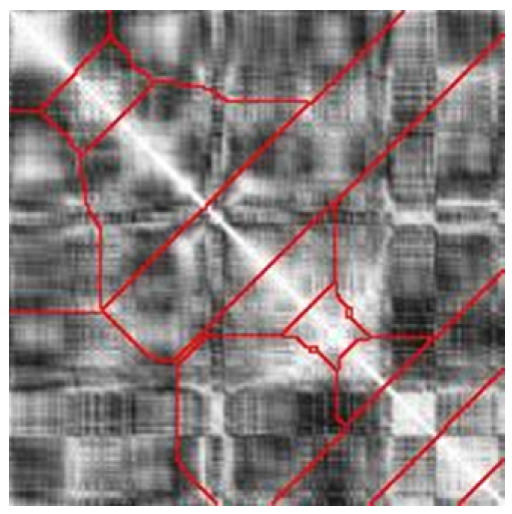
\includegraphics[scale=0.3]{images/chap2_watershed.png}
\caption{在類詞片段上進行的Watershed轉換,紅線部分為可能的次詞邊界} \label{fig:chap2_watershed}
\end{figure}


\section{遞迴式類神經網路語言模型}
\subsubsection{模型結構}
如圖 ~\ref{fig:chap5_rnn_structure} 所示,遞迴式類神經網路語言模型主要可以分為三個層級:
\begin{figure}
\centering
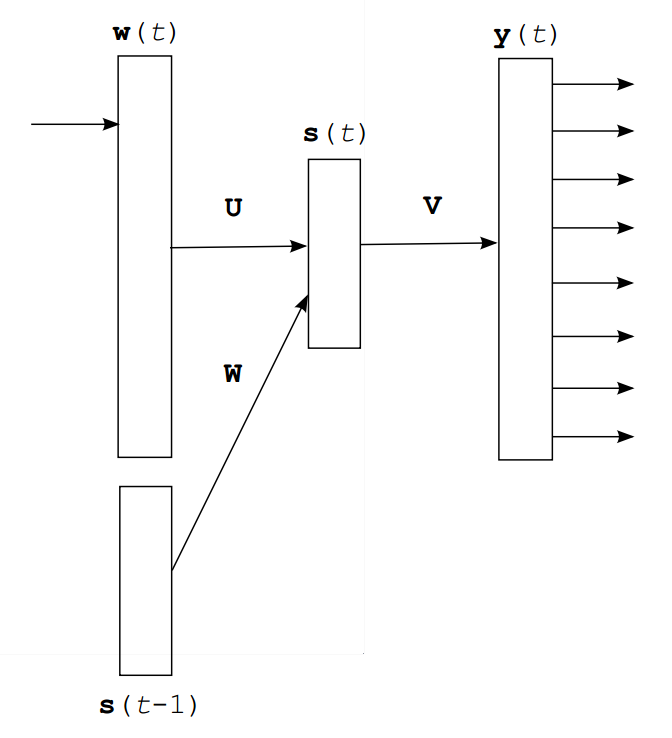
\includegraphics[scale=0.3]{images/chap5_rnn_structure.png}
\caption{遞迴式類神經網路語言模型示意圖} \label{fig:chap5_rnn_structure}
\end{figure}

1. 輸入層 (Input Layer):是一個與辭典大小同長度的陣列,採用的是1-of-N編碼 (1-of-N Encoding)形式,輸入為前一個詞在辭典裡的索引 $w(t)$,而只有該索引的位置的值為一,其餘皆為零。

2. 輸出層 (Output Layer):同樣是一個與辭典大小同長度的陣列,也是採用1-of-N編碼形式,代表的是該模型對下一個字出現機率分布的預測 $y(t)$。

3. 潛藏層 (Hidden Layer):或稱上下文層(Context Layer),通常維度較小,代表的是該時間點此模型保存的上下文資訊 $s(t)$。此層與輸入層、輸出層各有一組權重矩陣 (Weight Matrix) ,$\mathcal{U}$和$\mathcal{V}$,與上一個時間點的潛藏層向量 $s(t-1)$ 也存在一組權重矩陣 $\mathcal{W}$,其用意是為了模擬上下文間的相依關係。

有了以上三層與矩陣後,可以將輸入層、潛藏層及輸出層的關係表示如下:

\begin{equation}
s(t) = f(\mathcal{U}\times w(t) + \mathcal{W}\times s(t-1))
\end{equation}

\begin{equation}
y(t) = g(\mathcal{V}\times s(t))
\end{equation}

其中的$f(\cdot)$和$g(\cdot)$分別為邏輯函式 (Logistic Function) 與 Soft-Max 函式:

\begin{equation}
f(z) = \frac{1}{1+e^{-z}}
\end{equation}

\begin{equation}
g(z_m) = \frac{e^{z_m}}{\sum_k e^{z_k}}
\end{equation}

\subsubsection{最佳化演算法-沿時間反向傳播}
沿時間反向傳播的核心精神是基於反向傳播演算法 (Back Propagation) 而來,反向傳播演算法是訓練類神經網路 (Neural Network) 的最佳化演算法,而反向傳播演算法主要的步驟包含了以下三個部分:

1. 給定一筆訓練範例 (Training Example) 及現階段的模型參數組合,從輸入層向輸出層做順向傳遞 (Forward Pass) ,輸出現階段模型的預測結果 $y_j$,$0<j<|V|$。

2. 根據第一步中模型的輸出結果 $y_j$,與真正的結果 $d_j$ 間計算誤差值,在語言模型中誤差函數 (Error Function) 為交叉熵 (Cross Entropy):

\begin{equation}
\label{equ:chap5_error_function}
E = \sum_j d_j \log{y_j}
\end{equation}

3. 根據第二步算出來的誤差函數,計算其一階倒數 (First Derivative),調整進來的權重 (Incoming Weight),並重複將這個誤差訊號利用連鎖法則 (Chain Rule) 往前傳遞,直到傳回輸入層為止。

假設$y_j$與$z_j$分別是輸出節點$j$的輸出訊號與輸入訊號,$y_i$是潛藏節點 $i$ 的輸出訊號。其中$y_j=f(z_j)$經過一個激活函數 (Activation Function) $f(\cdot)$轉換。假設已知誤差函數為式 ~\ref{equ:chap5_error_function},我們就可以計算它對$y_j$的一次偏微$\frac{\partial E}{\partial y_j} = \frac{d_j}{y_j}$,根據連鎖法則,即可推得:

\begin{equation}
\frac{\partial E}{\partial z_j} = \frac{\partial E}{\partial y_j} \frac{y_j}{z_j} = f^{'}(z_j) \frac{\partial E}{\partial y_j}
\end{equation}

且:
\begin{equation}
\frac{\partial E}{\partial y_i} = \sum_j \frac{\partial E}{\partial z_j} \frac{\partial z_j}{\partial y_i} = \sum_j w_{ij} \frac{\partial E}{\partial z_j}
\end{equation}

故我們可以推得誤差函數 $E$ 對權重 $w_{ij}$ 的一階導數:

\begin{equation}
\frac{\partial E}{\partial w_{ij}} = \frac{\partial E}{\partial z_j} \frac{\partial z_j}{\partial w_{ij}} = y_i \frac{\partial E}{\partial z_j} 
\end{equation}

而此值就被拿來當作梯度下降法 (Gradient Decent) 中更新權重 $w_{ij}$ 的依據。

沿時間反向傳播演算法~\cite{boden2002guide}是由反向傳播演算法而來,其唯一不同之處是在做模型訓練之前,必須根據所設定的展開時間層數,將潛藏層往前展開 $N$ 層,圖 ~\ref{fig:chap5_bptt}
中顯示的是將潛藏層往前展開三層的結果。展開之後其實相當於訓練兩個前饋式類神經網路,一為圖中的上半部,包含輸出層、原始潛藏層及輸入層,另一為圖中的下半部,包含所有沿時間展開的潛藏層及其對應的輸入層。另一方面,由於模型有隱含序列的特性,因此在訓練的過程中必須保持序列的順序一筆一筆餵入作訓練。訓練後各時間點的潛藏層與潛藏層間的權重矩陣將被取平均,以讓各時間點的權重相同。

\begin{figure}
\centering
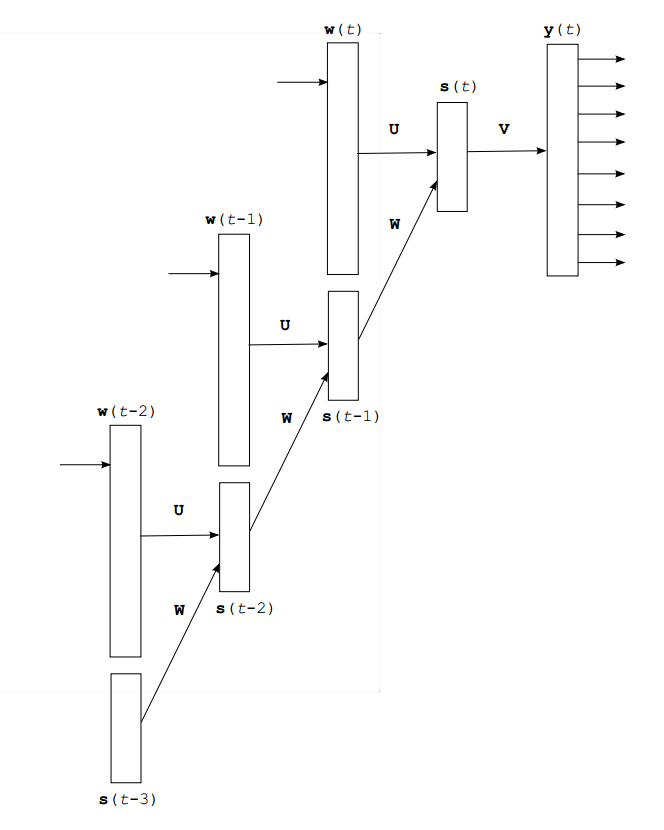
\includegraphics[scale=0.5]{images/chap5_bptt.png}
\caption{將潛藏層向前展開三層的示意圖} \label{fig:chap5_bptt}
\end{figure}

\section{本章總結}
本章介紹了資訊檢索的背景,包含了基礎的資訊檢索架構、口述語彙偵測與語意檢索的差別,以及相關回饋的基本概念,並介紹了語音檢索系統的兩個主要的部分:辨識系統與檢索系統,最後介紹了動態時間校準做為口述語彙偵測的方法。
